%
%                       This is a LaTeX 2e version of the
%                       laboratory project template file.
%\documentclass{aa}
\documentclass[a4paper,12pt]{article}
%\usepackage{fullpage,epsf}
%
%                       This subsection generates a title page
%                       Edit only the subsections indicated to put
%                       in the project title, your name, supervisor,
%                       project length in weeks and submission date
\usepackage[english]{babel}
\usepackage[utf8]{inputenc}
\usepackage{csquotes}% Recommended
\usepackage{amsmath,amssymb,latexsym}
\usepackage{graphicx}
\usepackage{subfig}
\usepackage{geometry}
\usepackage{lipsum}
\usepackage{epigraph}

\setlength{\parindent}{2em}
%\setlength{\parskip}{1em}
%\usepackage{biblatex}
\usepackage{natbib}
\usepackage{aas_macros}
%\bibliographystyle{agsm}
\usepackage[nottoc,notlof,notlot]{tocbibind} 
\renewcommand\bibname{References}
\bibpunct{(}{)}{;}{a}{}{,} % to follow the 
\usepackage{listings}
\usepackage{color}

\definecolor{dkgreen}{rgb}{0,0.6,0}
\definecolor{gray}{rgb}{0.5,0.5,0.5}
\definecolor{mauve}{rgb}{0.58,0,0.82}

\lstset{
  language=Python,
  aboveskip=3mm,
  belowskip=3mm,
  showstringspaces=false,
  columns=flexible,
  basicstyle={\small\ttfamily},
  numbers=left,
  numberstyle=\tiny\color{gray},
  keywordstyle=\color{blue},
  commentstyle=\color{dkgreen},
  stringstyle=\color{mauve},
  breaklines=true,
  breakatwhitespace=true,
  tabsize=3,
  frame=single
}

\begin{document}
\pagestyle{empty}                       % No numbers of title page                      
%\epsfxsize=40mm                         % Size of crest
\begin{minipage}[b]{110mm}
        {\Huge\bf Computer and \\Information Sciences
        \vspace*{17mm}}
\end{minipage}
\hfill
\begin{minipage}[t]{40mm}               
        \makebox[40mm]{
        
\includegraphics[width=1\linewidth]{strath_logo.png}}
\end{minipage}
\par\noindent                                           % Centre Title, and name
\vspace*{0cm}
\begin{center}
        \Large\bf \Large\bf Dissertation\\
        \Large\bf MSc Software Development\\[10pt]                     % Change to MP/CP/Astro
        \LARGE\bf Automated Mutation Testing for Concurrent Software         % Change to suit
\end{center}
\vspace*{0cm}
\begin{center}
        \bf Patrick Gray\\                           % Replace with your name
        August 2019                                    % Submission Date
\end{center}
\vspace*{5mm}
%
%                       Insert your abstract HERE
%                       
\begin{abstract}

\end{abstract}
\vspace*{2cm}
Signature:\hspace*{8cm}Date: 19/08/2019

\vfill
{\bf Supervisor:} Kostas Liaskos             % Change to suit
\hfill
                                       % Change to suit
\newpage

%
%                       End of Title Page
\pagestyle{plain}                               % Page numbers at bottom
\setcounter{page}{1}                            % Set page number to 1
\tableofcontents                                % Makes Table of Contents

\newpage
\section{Introduction}

\newpage
\section{Background}

The relevant background information required for this project will be presented here, as well as a review of the literature covering concurrent bug patterns and mutation operators. An overview of concurrency in Java and mutation testing for general software will provide the necessary understanding for the motivation of this project.  


\subsection{Concurrency}
\subsubsection{Threads}

Processes are self contained execution environments with private resources; most Java applications only require a single process to run efficiently. Modern computer systems provide multiple cores to process parallel execution of processes. Concurrency utilises this functionality with the use of \textit{Threads}. Threads are light-weight processes that share their resources (memory, open files, etc) with the other threads contained within the process \citep{mois15}. With the advancement of technology producing evermore powerful machines, each individual core has the ability to interleave multiple threads as well as the capability of running threads in parallel on separate cores. 

Creating threads is lighter on resources than creating new processes and the ability to share resources is beneficial to performance. This is the main motivation for using concurrent code; allowing multiple sections of code to run simultaneously for faster execution times. Another positive aspect of this is the improved responsiveness of a system \citep{peierls05}. When one section of a program becomes blocked or slows down, a single threaded system would become unresponsive to the user and would report no information back to explain why. A multi-threaded application would allow a computationally greedy operation to perform in the background without disrupting the rest of the system and remaining responsive to observation and interaction from the user.

Each program has at least one thread, the main thread, created at point of calling the main() method, but subsequent threads can be created after this execution. There are two ways to create new instances of threads. The first is to create an object that has implemented the Runnable interface and pass this to the Thread constructor. The thread will then execute the run() method of the runnable object. The other is to create an object that is a subclass of Thread and executing the run() method pertaining to the object \citep{oracle19}. In both cases, Thread.start() must be executed to start a specified instance of a thread. Although, threads are not necessarily run in the order of their start() execution, the threads are automatically assigned a priority by the Java Vitrual Machine (JVM), and scheduled in order of highest priority \citep{mois15}. The first instance is a more general and flexible approach since it is implementing the Runnable interface, it allows for the class to inherit functionality from another class. This also has the benefit of allowing its own parameters to be passed to the constructor. The second is easier to use in simple applications, but since it is a subclass of Thread, there are limitations to what the class can do, as only the parent class Thread constructors are available. 

If a thread wants another thread to stop then it can invoke an interruption using Thread.interrupt(), which will throw an exception message to the interrupted thread. A thread can support its own interruption by invoking the sleep() method to stop itself for a specified period of time. After the elapsed time, the thread will resume running, unless an interrupt is called and the thread is terminated. Sleep() can be used by the user to manage the scheduling of threads if it is prescient for a particular operation and limits the unpredictability of the system behaviour. Similar to a thread sleep, Thread.join() can be used for one Thread to wait until another has completed its execution. With no specified time, the Thread may wait indefinitely for the other one to terminate. 


\subsubsection{Atomic Operations}

An atomic operation is one that is executed and completed all at once or not at all \citep{oracle19}. It is an action that is considered safe from interference from other operations, as it cannot be stopped during execution and the state of the process cannot be changed by another operation: the state is only affected by the atomic operation from the start to finish. A single line of code does not imply atomicity, no matter how deceptively simple it may appear. For instance, the increment operation for some integer, x++, is actually three separate operations handled by the Java Virtual Machine. First the value of the integer must be fetched, then it is incremented and finally the new value is written back to memory. This may seem trivial, but if mishandled, this can have unexpected and varying results if it is executed in conjunction with another Thread that is accessing the same data. When two threads interleave in such a way, it is referred to as interference. As an example, Thread A and Thread B are tasked to perform the increment operation on x. If they were to run consecutively, allowing for complete execution of the first operation before the initiating the next, the value of x would be expected to have increased by 2. However, if the two operations are executed at the same time, the following scenario could feasibly occur:
\begin{enumerate}
    \item Thread A retrieves the value of x, x = 0.
    \item Thread A increments x, x = 1.
    \item Thread B retrieves the value of x before the Thread A has been given the chance to commit the change of x to memory and thus, x remains equal to 0.
    \item Thread A stores the result of x = 1.
    \item Thread B increments x to 1 and stores the result. Despite two instances of incrementing the value of x, the final value is recorded as 1; the first instance has been overridden by the second.
\end{enumerate}

\begin{table}[]
    \centering
    \begin{tabular}{||l c||} 
     \hline
     Operation & Value of x  \\ 
     \hline\hline
     Thread A retrieves x & 0 \\ 
     \hline
     Thread A increments x & 1  \\
     \hline
     Thread B retrieves x & 0 \\
     \hline
     Thread A stores value of x & 1 \\
     \hline
     Thread B increments x & 1 \\  
     \hline
     Thread B stores value of x & 1 \\
     \hline
    \end{tabular}
    \caption{Example of a non-atomic operation, x++, in two interleaving threads.}
    \label{table:non-atomic}
\end{table}

 

This is only one small example of interference, but similar occurrences of inconsistent memory issues between threads can crop up throughout concurrent systems unless properly managed. Compounding this is the complexity of other scenarios with a greater number of interleaving threads and manipulation of more data. One method of preventing this is utilising the functionality of synchronized code, which will be explored in the following section.


\subsubsection{Synchronization and Locks}
    
Synchronisation allows for critical sections of code or methods to be executed atomically with reference to code in other threads. The power of scheduling operations and resource management is passed to the user \citep{silberschatz13}. The synchronized keyword blocks other threads from executing simultaneously during its execution to ensure that the state of the system is only affected by the actions within the synchronized block. Synchronization can be applied to a specific set of actions in a block, specifying the resource to be restricted or to an entire method. The two methods of using the synchronized keyword are shown in Figure \ref{fig:synchronized}. 

\begin{figure}[h]
    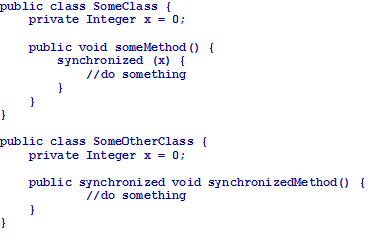
\includegraphics{synchronized.png}
    \caption{Synchronized blocks}
    \label{fig:synchronized}
\end{figure}

Restricting the whole method will have a more dramatic effect on the performance as no other threads can run concurrently. Applying synchronization to the increment example would solve the observed problem of memory consistency and would guarantee the expected result to occur.

The synchronized keyword achieves the desired affect by imposing a lock on the synchronized block of code that prevents access to the contained object’s fields. After the synchronized block has terminated, the lock is released and normal thread scheduling will resume. Reentrant locks can be used to similar effect to the synchronized keyword, allowing a thread to obtain and release a lock during execution of critical code, much like a synchronized block of code. 

\subsubsection{Liveness}
The liveness of an application expresses its ability to execute without complications in an efficient manner. There are some issues that can interfere with the liveness of an application by slowing it down or even freeze functionality altogether. A deadlock can occur when two threads have locked separate resource, but are waiting on the other thread to release their lock to continue execution. 

\vspace{2pt}
\begin{center}
\noindent Thread 1: locks resource A, waits for resource B
\\Thread 2: locks resource B, waits for resource A 
\end{center}
\vspace{2pt}

In this instance, both resources are locked and unavailable for access until the other is released; the program will perpetually hang in an inescapable catch-22.  


\subsubsection{Executor Service}
Previously, concurrency examples provided have only involved two threads that are relatively simple to follow. In many cases, a program may wish to utilise many more threads for a significant boost in performance. The Java concurrent package offers the Executor Service to help maintain many instances of threads, a thread pool, by abstracting the management and construction of threads from the main program. This can be an invaluable tool for ensuring computation resources are not wasted by the constant creation of new threads for each concurrent action. Instead, a pool of threads is created at once and the threads will wait until they are required. After performing the necessary action, the thread will go back into a state of waiting for a request for work. The size of the pool has a specified limit, to prevent a runaway of thread creation; when all the threads in a pool are currently in use, the executor server will wait to assign work to the next available thread. Creating a thread takes up time and resources, it is far more efficient to recycle previously used threads. 



\subsection{Mutation Testing}
Mutation testing is the process of seeding errors throughout a system’s codebase, to observe the effecting behaviour and evaluate the effectiveness of the present testing coverage. The premise is simple: if the tests have been designed adequately, then they should recognise the changes to the system behaviour and certain tests should fail accordingly. The mutation is referred to as killed in this instance. This is the ideal outcome when a mutation is applied to a system, as it suggests that the tests have been designed effectively and the coverage is sufficient. However, if a mutation survives by circumventing the tests, this indicates that the tests are either flawed or the test coverage has gaps and not all of the behaviour has been accounted for. This is a useful tool for highlighting weaknesses in test coverage; a full suite of unit tests that successfully pass when run on a system only informs the user that those specific function behaviours are expected. Although it provides no information on the behaviours that have been missed. Mutation testing aides identifying these areas of code that have been overlooked by applying many different mutations throughout the whole system, which should disrupt as much expected behaviour as possible. Thus, when a mutation is not successfully killed by any unit test, the location of the altered code will indicate that there is improvement to be made in the test coverage related to the affected area.

There are many different mutation testing tools available: Pitest (PIT) being the most renowned for Java \citep{pit19}. PIT combines traditional line coverage with mutation coverage, to offer a comprehensive and fast testing environment for Java applications. The list of mutation operators is extensive, covering relational operators (e.g. \textless, \textless=, \textgreater, \textgreater=), mathematical operators (e.g. +, -, *, etc.), logic statements a variety of different common method calls and return values \citep{pit19}. A mutation usually consists of altering a small section of code or removing a section entirely. For example, a conditional boundary operator would make the following mutation  in Figure \ref{fig:mutation}. 

\begin{figure}[h]
    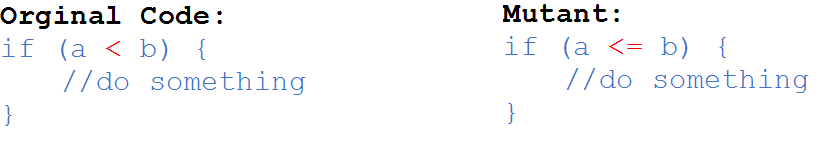
\includegraphics{mutation.png}
    \caption{Relational operator mutation}
    \label{fig:mutation}
\end{figure}
    
The code now has a slightly different meaning. Designing effective unit tests involves specifically testing code at such boundary cases. The behaviour of the code would be monitored for values of a when less than b, equal to b and greater than b, with a separate test for each scenario. Prior to the mutation, the if statement would not be executed during runtime for when a is equal to b, but after the mutation the if statement would be entered. Thus, a unit test that previously would pass for this scenario should fail due to the alteration and the mutation could be considered successfully killed. PIT will apply many of these mutations on the byte code generated after compilation, instead of on the source files. This produces significantly faster runtimes. After mutation, PIT will automatically run the new java files against the designated unit tests and produce a set of results detailing the fates of each mutation. The varying states explained below:

\begin{description}
    \item[Killed - ]The mutation was successfully discovered by the presence of a failed unit test.
    \item[Lived -]The mutation was unsuccessfully discovered with no failed unit tests. 
    \item[No coverage -]The mutation lived because of a lack of unit tests covering the relevant mutated section of code. 
    \item[Non-viable -]The mutation affected the Java bytecode such that the JVM could not load the file.
    \item[Timed out -]The mutation created an infinite loop so execution of the file could not terminate. 
    \item[Memory error -]The mutation increased “the amount of memory used by the system or the result of the additional memory overhead required to repeatedly run your tests”.
    \item[Run error -]The mutation caused the file to be unable to run, similar to non-viable mutations.
\end{description}

The results detail which mutations were applied, identify which tests managed to kill mutations and produce the ratio of successfully caught mutations to the total number of seeded errors. Although PIT offers a wide range of mutation operators, it is lacking in support for concurrent systems. Performing unit tests on multi-threaded code is not as straightforward as single threaded [unclear why].
    

\subsection{Concurrent Bug Patterns}
    
    
    
\subsection{Mutation Operators}
\citet{bradbury06} have comprehensively designed a set of mutation operators specific to the concurrent functionality and the bug patterns identified by \citet{farchi03}. The focus of their research is in response to the updated concurrent functionality introduced in the J2SE 5.0 version of Java. Synchronization can now be implemented using explicit locks, semaphores, barriers, latches and exchangers. Support for these various concurrent operations persists through the more recent versions of Java with some minor updates and revisions. In total, \citeauthor{bradbury06} to produce 22 different mutation operators, each of which are associated with a number of different concurrent methods. The operators are split into groups relating to a concurrent bug pattern found in the work of \citeauthor{farchi03}.


\subsection{Parsing/Regular Expressions}



\newpage
\section{Methodology}
\subsection{Mutation Operators}

MXT – Modify Method-X Timeout
\\MSP – Modify Synchronized Block Parameter
\\RTXC – Remove Thread Method-X Call
\\RCXC – Remove Concurrency Mechanism Method-X Call 
\\RNA – Replace NotifyAll() with Notify()
\\RJS – Replace Join() with Sleep()
\\RSK – Remove Synchronized Keyword from Method
\\ASTK – Add static keyword to method
\\RSTK – Remove Static Keyword from Method
\\RVK – Remove Volatile Keyword
\\RFU – Remove Finally Around Unlock

The automatic mutation application tool currently only supports application of four of these mutation operators with all of the relevant concurrent keywords and methods: MXT, MSP, RTXC and RCXC. However, at least 7 more of the operators could be implemented with little difficulty due their similar mechanisms. The regular expression used is very consistent for simple removals of keywords and minor modifications to method parameters. The operators that have been implemented already were chosen based on the needs of the banking system and the limited number of concurrent methods present in the code.   
	
	
	
	
	\subsection{Mutation Tool}
	\subsection{Concurrent Software}
	    \subsubsection{Banking System}
	    \subsubsection{Incrementer System}
	\subsection{Unit Tests}
	    \subsubsection{JUnit Tests}
	    \subsubsection{Concurrent Tests}
    \subsection{Software Engineering}
	
	
\newpage	
\section{Analysis}
    \subsection{Results}
    \subsection{Results Analysis}

Bradbury et al. conjecture that “The MXT operator with the sleep() and join() methods is most likely to result in the sleep() bug pattern… where a sleep() or join() is used by a caller thread to wait for another thread, reducing the time may cause the caller thread to not wait long enough for the other thread to complete.  

“The MXT operator when applied to an await method call will most likely result in an interference bug” – compare actual results to their hypotheses.

“The MSP operator will result in the wrong lock bug pattern”

“The ESP mutation operator can result in a wrong lock bug because exchanging two adjacent locks will cause the locks to be acquired at incorrect times for incorrect critical regions. The ESP operator can also cause a classic deadlock (via deadly embrace) bug to occur as is the case in the above example.”

“Removing the wait() method can cause potential interference, removing the join() and sleep() methods can cause the sleep() bug pattern, and removing the notify() and notifyAll() method calls is an example of losing a notify bug.”

“The RCXC operator removes this [unlock] call thus the lock is not released. This is an example of a blocking critical section bug.”

    
    
    
    
    \subsection{Methodology Analysis}

The incrementer system has been designed to purposefully encounter concurrent problems, such as thread interference and memory consistency errors. The reason behind this is to easily catch the bugs that are present after a mutation has taken place in one of the system class files. Await() and sleep() statements were utilised to slow down the computation time and increase the likelihood of two threads attempting to access state variables within the same window. This serves as a proof of concept that it is possible and fairly straightforward to design effective unit tests for concurrent code. Although, obviously, in real-life scenarios, compromising the performance and execution time of large systems is not ideal. Especially considering the main motivation of implementing concurrency to a system is to improve the performance. The test environment can be used to determine whether the system has been properly safeguarded with less concern for efficiency.

There may be an argument to introduce a default wait time of 0 seconds, stored as a variable, to be used as a parameter for the relevant methods, so that in normal use the system will function with the desired efficiency. However, when it comes to testing, this variable can be altered to a more suitable value that will provide significant opportunity for errors to arise that would remain hidden in the default state of execution. 

It was deemed sufficient to test the systems with only two threads. Since the systems were small in scale and designed in such a manner that errors would be readily caught, increasing the number of threads would be superfluous. If a mutation was identified and killed by any unit test with only two interleaving threads, then the mutation would definitely be caught in number of more threads. However, in larger, more complex systems, any bug may be significantly harder to find, so increasing the number of threads with the objective of maximising the likelihood of interference could be an effective approach.

    
    
\newpage	
\section{Conclusion}

\subsection{Future Work}
The original goal was to end up with a full test suite that would seed many mutations throughout the code, perform the unit tests and produce a set of results. The results would detail which mutations were applied, identify which tests managed to kill mutations and produce the ratio of successfully caught mutations to the total number of seeded errors. Due to time limitations, a revision of expectations and priorities, the focus was on developing the mutation system and the unit tests for the sample test systems. Thus, many of the stages above were carried out manually. A complete automatic tool for evaluating the effectiveness of concurrent tests would be a valued area for future development. The inspiration for the tool described was spawned from the presence of other mutation testing tools, such as Pitest, which provides a full mutation testing environment and many operators to select. However, none of the available tools provide support for concurrent operators due to the special difficulties that surround the subject.
    
\newpage
\section{Acknowledgements}

\bibliographystyle{agsm} % style aa.bst
\bibliography{bibliography.bib}

\newpage
\appendix
\section{Appendices}


\end{document}
